\chapter{Experiments and Results}\label{Chapter:experiments}


\section{Lookup Tables} \label{datasets:lt}

The lookup tables task was introduced by \cite{Liska2018} within the CommAI domain \citep{Baroni2017} as an initial benchmark to test the generalization capability of a compositional learner. The data consists of atomic tables which bijectively map three bit inputs to three bit outputs. The compositional task can be understood in the form of a nested function $f(g(x))$ with $f$ and $g$ representing distinct atomic tables. To clarify the task with an example, given $t1$ and $t2$ refer to the first two atomic tables respectively; also given that $t1(001) = 100$ and $t2(100) = 010$. Then a compositional task is presented to a learner as $001 t1 t2 = 010$. Since the i/o strings are three bit, there can be a maximum of 8 input/output strings.

As is very clear from the task description that since the table prompts $t_i$ don't have any semantic meaning in itself, the meaning of each individual table prompt can be correlated only with the bijective mapping it provides. Secondly the dataset is in agreement with the systematic compositionality definition that we have outlined in section \ref{systematic}. Lastly one can argue that even a human learner might come up with an approach that is different than solving each function individually and sequentially in a given nested composition, but such an approach will not be able to scale with the depth of nesting.

\subsection{Data Structure}\label{lt:splits}
We generated eight distinct atomic tables $t1......t8$ and work with compositions of length two, i.e. $t_i - t_j$. This leads to a possible 64 compositions. Since we want our model to not simply memorize the compositions but rather to land on a compositional solution, we propose to use the compositions only from tables $t1 - t6$ for the training set. However since the model needs to know the mapping produced by tables $t7, t8$ in order to solve their compositions we expose the model to the atomic tables $t7, t8$ in the training set. The details of all the data splits and some dataset statistics are presented below. Examples from each split and the size of each split are presented in table \ref{lt:stats}

\begin{enumerate}
	\item \textbf{train} - The training set consists of the 8 atomic tables on all 8 possible inputs. The total compositions of tables $t1 - t6 = 36$. Out of those 36 compositions we take out 8 compositions randomly. For the remaining 28 compositions we take out 2 inputs such that the training set remains balance w.r.t. the compositions as well as the output strings. (Details of this sudoku algorithm in the appendix)
	\item \textbf{heldout inputs} - The 2 inputs taken out from the 28 compositions in training constitute this test set. However of the 56 data points, 16 are taken out to form a validation set. In creating this split we ensure that the splits i.e. \textit{heldout inputs} and \textit{validation} have a uniform distribution in terms of output strings at the expense of the uniformity in the compositions.
	\item \textbf{heldout compositions} - This set is formed by the 8 compositions that were taken out of the initial 36 compositions. These 8 compositions are exposed to all 8 possible input strings.
	\item \textbf{heldout tables} - This test is a hybrid of the tables which are seen in compositions during training i.e. $t1 - t6$ and those which are seen just atomically during training i.e. $t7 - t8$. There are total of 24 compositions in this split which are exposed to all 8 inputs.
	\item \textbf{new compositions} - This split consists of compositions of $t7 - t8$ and therefore a total of 4 compositions on 8 inputs.
\end{enumerate}


\begin{table}[ht]
	\centering
	\begin{tabular}{l|lc}
		& Example & Size\\
		\hline
		train & t1 t2 011 & 232 \\
		heldout inputs & t1 t2 001 & 40 \\
		heldout compositions & t1 t3 110 & 64 \\
		heldout tables & t1 t8 111 & 192 \\
		new compositions & t7 t8 101 & 32 \\
	\end{tabular}
	\caption{Lookup Table Splits}
	\label{lt:stats}
\end{table}


\begin{figure}[ht]
	\begin{subfigure}{0.5\linewidth}
		\ifpdf
		\includegraphics[width=0.95\linewidth]{./figs/lookup/train-pdf}
		\else
		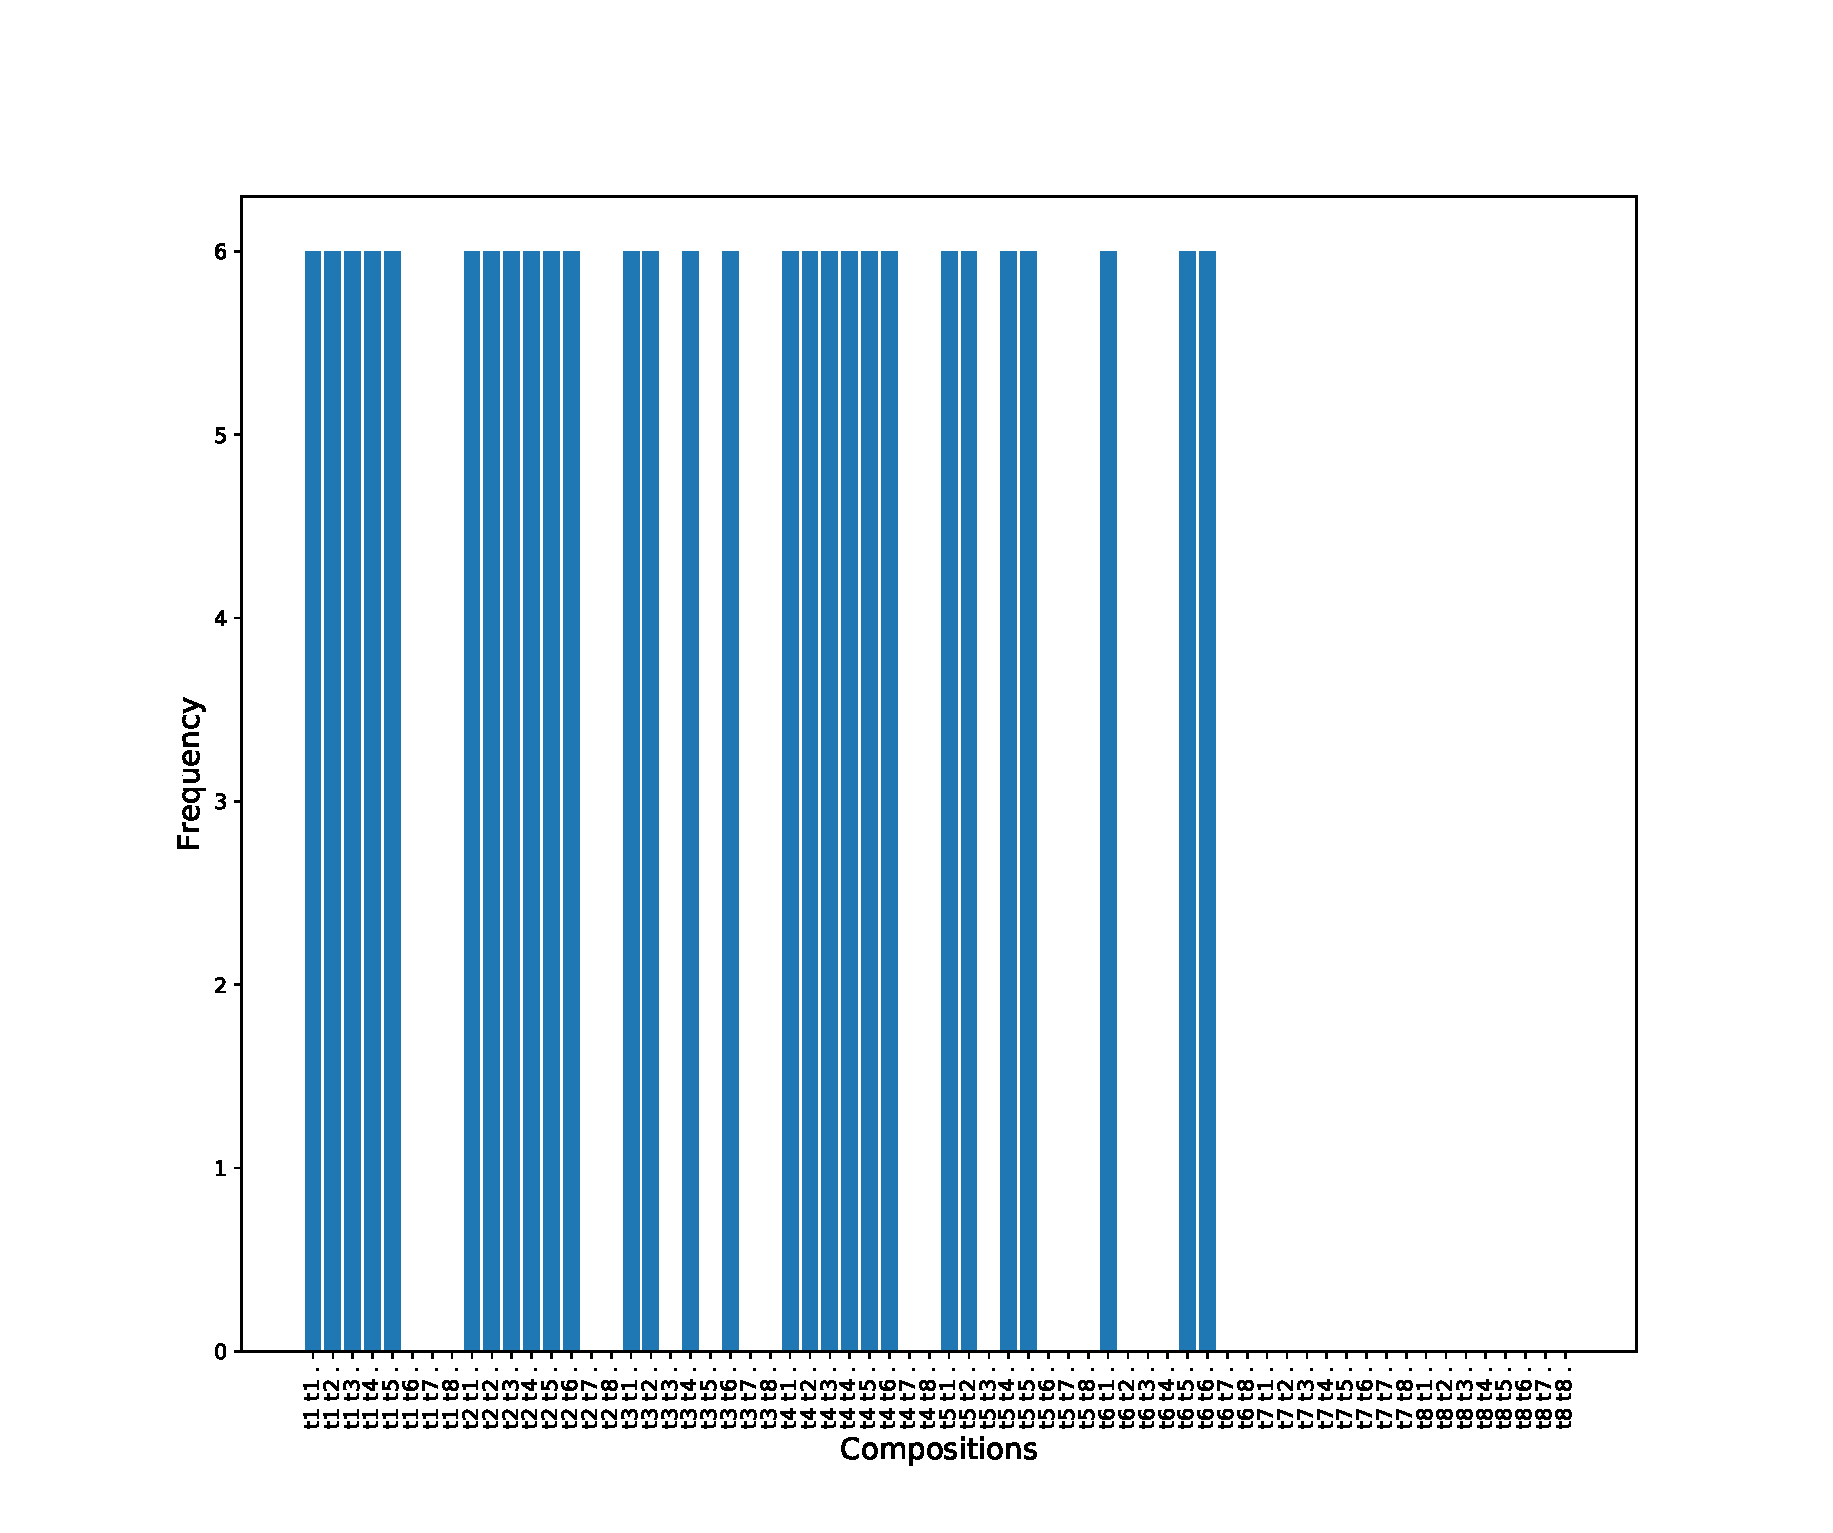
\includegraphics[width=0.95\linewidth]{./figs/lookup/train-eps}
		\fi
		\caption{Train}\label{fig:train_dist}
	\end{subfigure}
	\begin{subfigure}{0.5\linewidth}
		\ifpdf
		\includegraphics[width=0.95\linewidth]{./figs/lookup/heldout_compositions-pdf}
		\else
		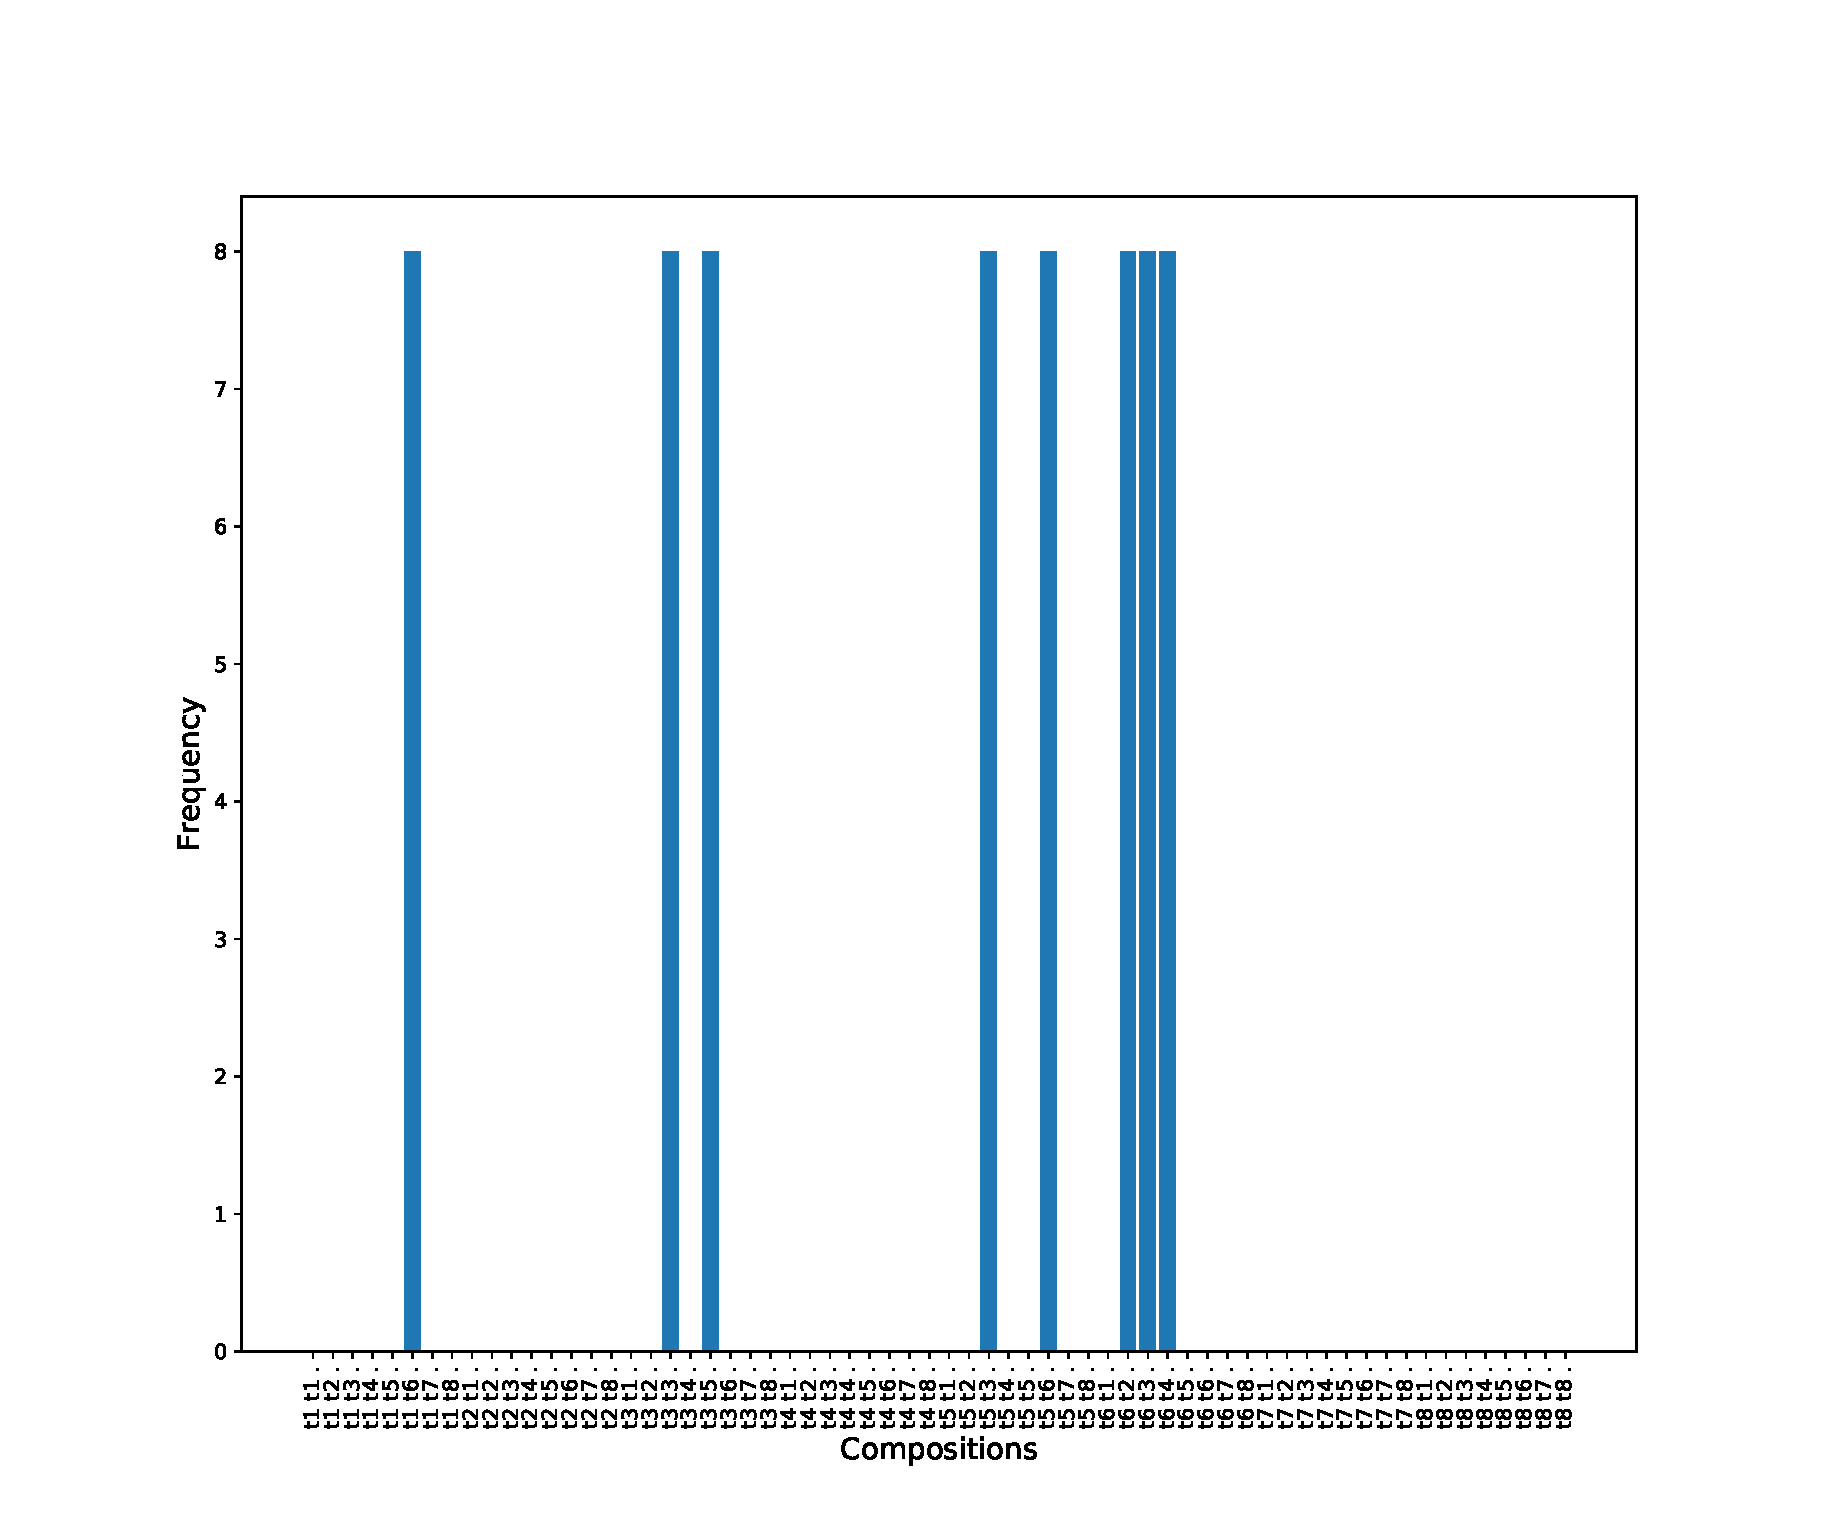
\includegraphics[width=0.95\linewidth]{./figs/lookup/heldout_compositions-eps}
		\fi
		\caption{Heldout Compositions}\label{fig:held_comp}
	\end{subfigure}
	\begin{subfigure}{0.5\linewidth}
		\ifpdf
		\includegraphics[width=0.95\linewidth]{./figs/lookup/heldout_tables-pdf}
		\else
		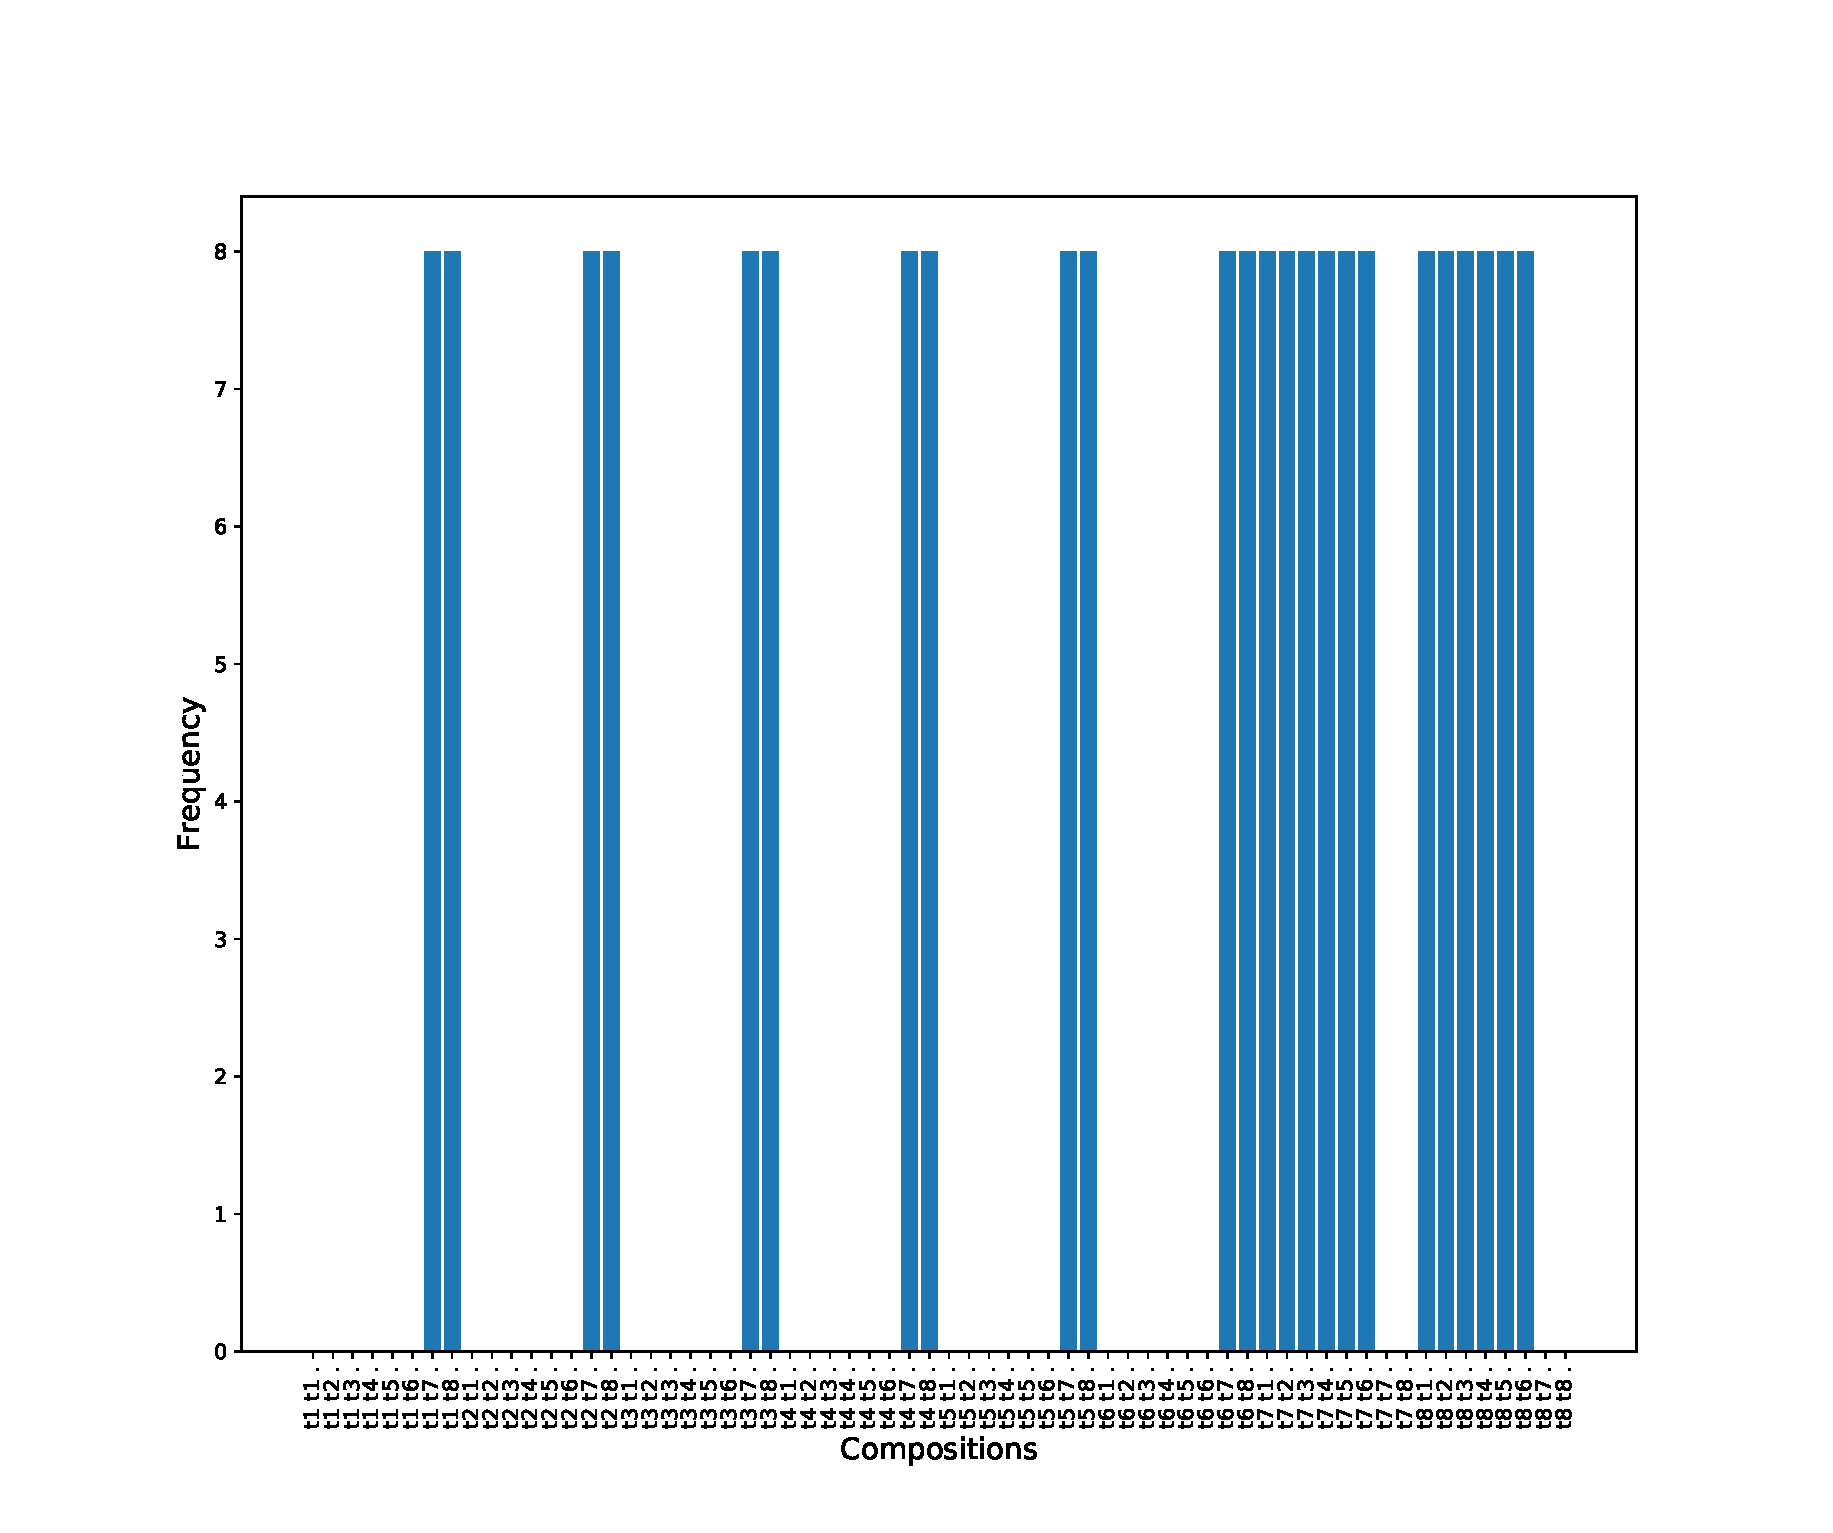
\includegraphics[width=0.95\linewidth]{./figs/lookup/heldout_tables-eps}
		\fi
		\caption{Heldout Tables}\label{fig:held_tab}
	\end{subfigure}
	\begin{subfigure}{0.5\linewidth}
		\ifpdf
		\includegraphics[width=0.95\linewidth]{./figs/lookup/new_compositions-pdf}
		\else
		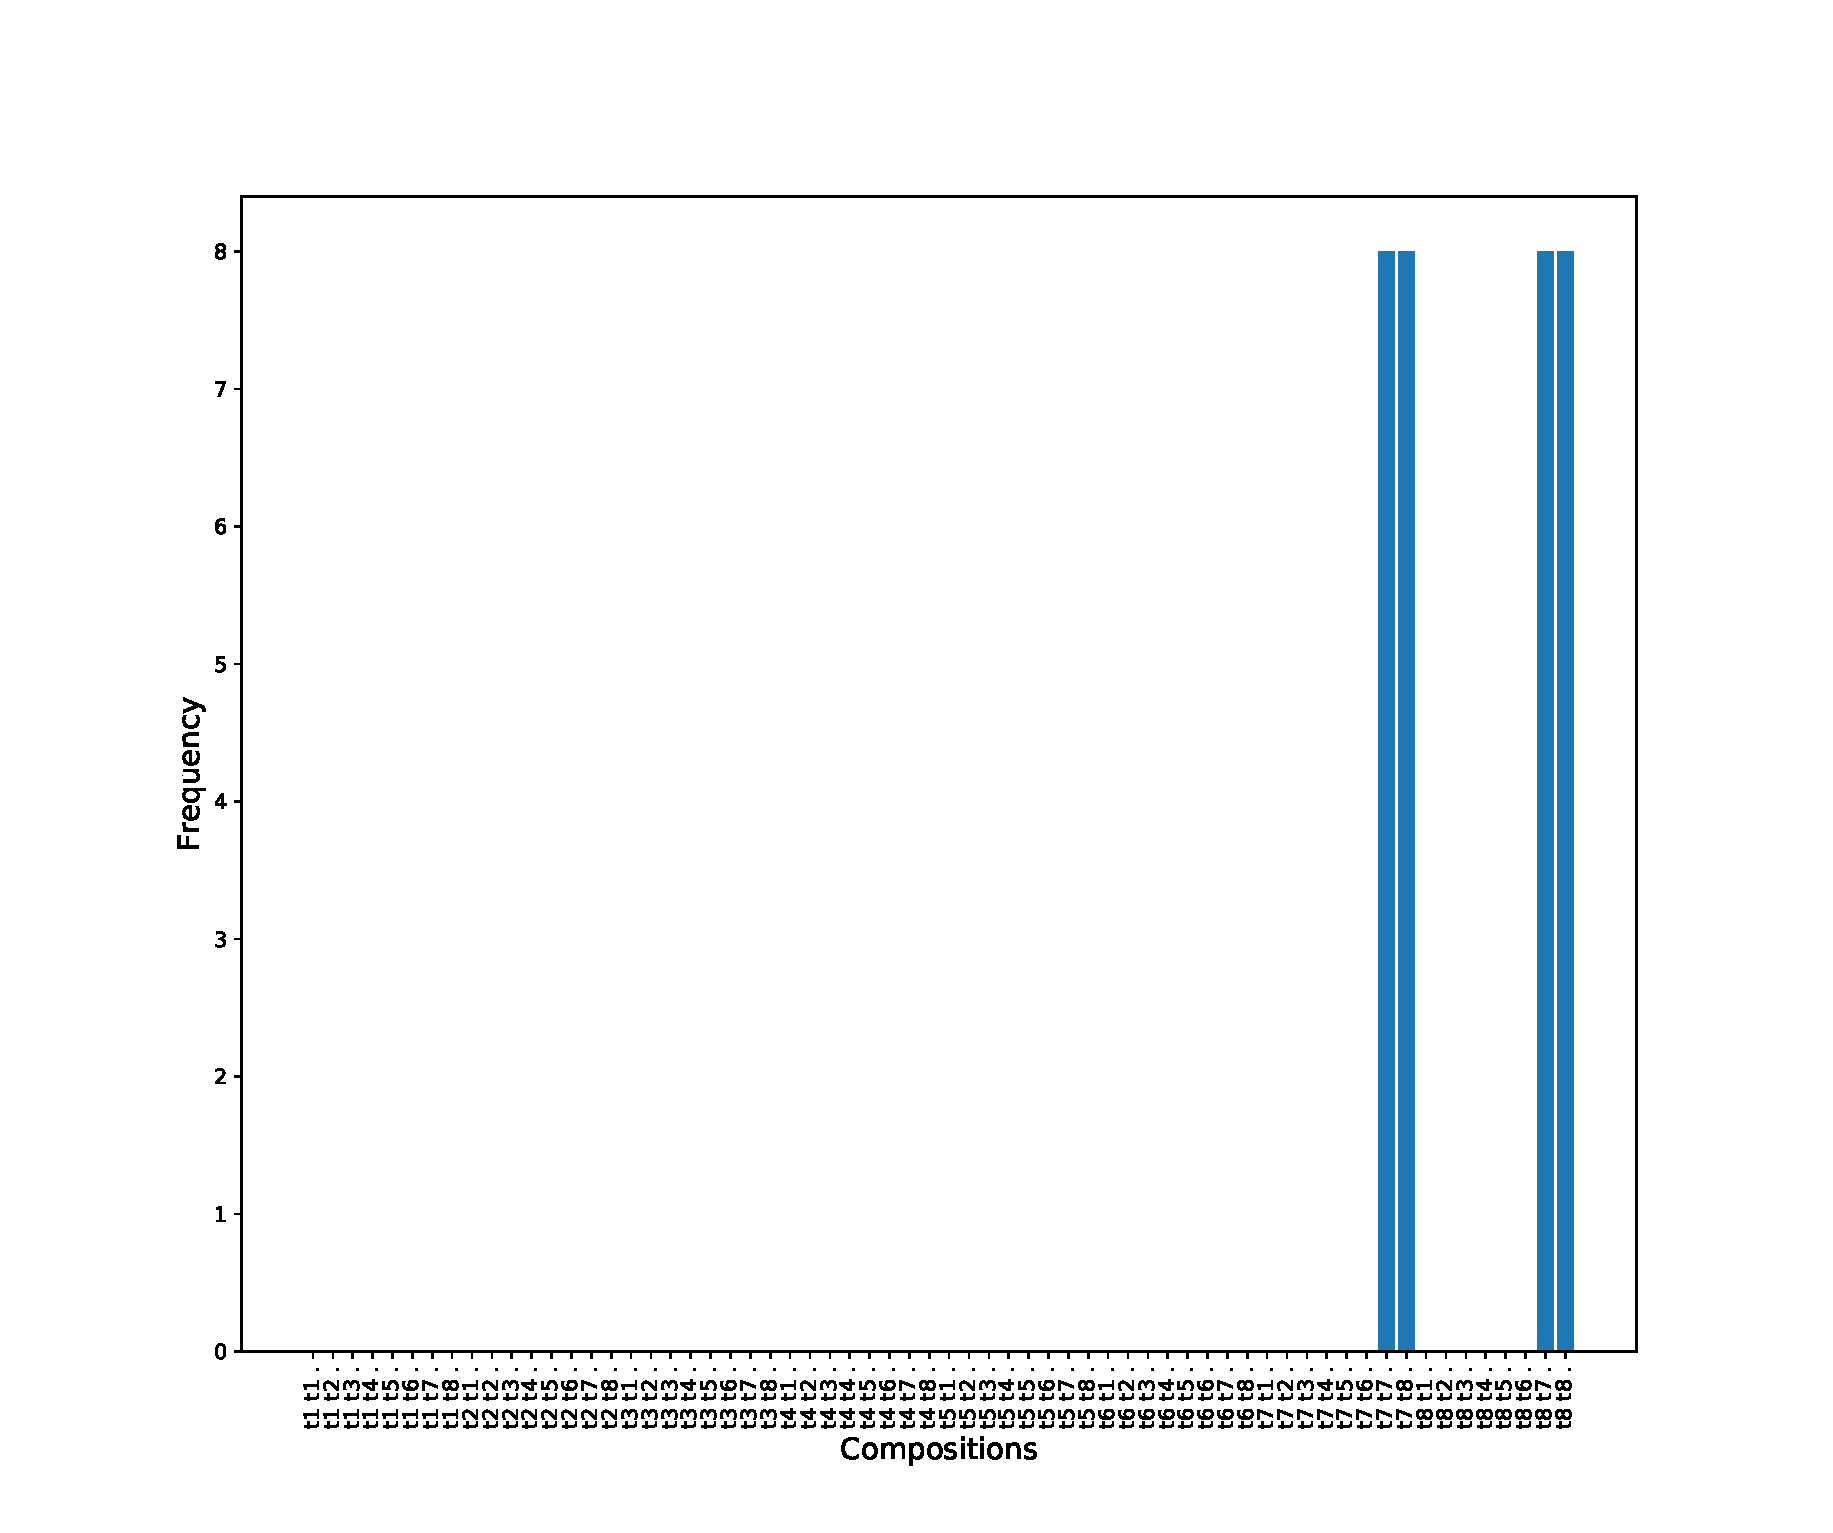
\includegraphics[width=0.95\linewidth]{./figs/lookup/new_compositions-eps}
		\fi
		\caption{New Compositions}\label{fig:new_comp}
	\end{subfigure}
	\caption{Data distribution of train and test sets}\label{fig:all_data}
\end{figure}
%, trim={15mm, 5mm, 35mm, 15mm}, clip
In accordance with the data split described above we present the distribution of all compositions in the train and various test sets. It can be seen that the test sets \lq heldout\_tables\rq{} and \lq new\_compositions \rq{} are the most difficult and require zero-shot generalisation owing to their significantly different distribution as compared to \lq train \rq{}.

\subsection{AG Trace}
As explained in section \ref{pm:ag-ponder} attentive guidance can help in mocking the pondering. For a lookup table composition of the form \lq $((000)t3)t1$ AG enforces pondering as follows:
\begin{equation}
t1(111) = 100 \qquad t3(000) = 111 \qquad ((000)t3)t1 = 100,
\end{equation}
the composed function is expanded as follows:
\begin{equation}
000\ t3\ t1 = 000\ 111\ 100.
\end{equation}
AG therefore forces the decoder to ponder for two additional steps. The biggest difference from the Pondering in section \ref{mtv:ponder} would be that at each pondering step we have an emission, instead of the ponder step being a silent one. The trace for the attentive guidance can be explained as follows and is shown in figure \ref{ag_lt}:
\begin{itemize}
	\item The first step is the copy step where the three bit input to the composition is copies as if.
	\item After this the tables in the composition are applied sequentially to the three bit input preceding them.
	\item The diagonal trace is mean to capture this sequential and compositional solution of lookup tables. At each step of decoding we force the model to focus on only that input prompt which results in the correct output for that step.
\end{itemize}

\begin{figure}
	\begin{minipage}[t]{\textwidth}
		\ifpdf
		\includegraphics[width=\linewidth,keepaspectratio=true]{./figs/lookup/lt-trace-pdf}
		\else
		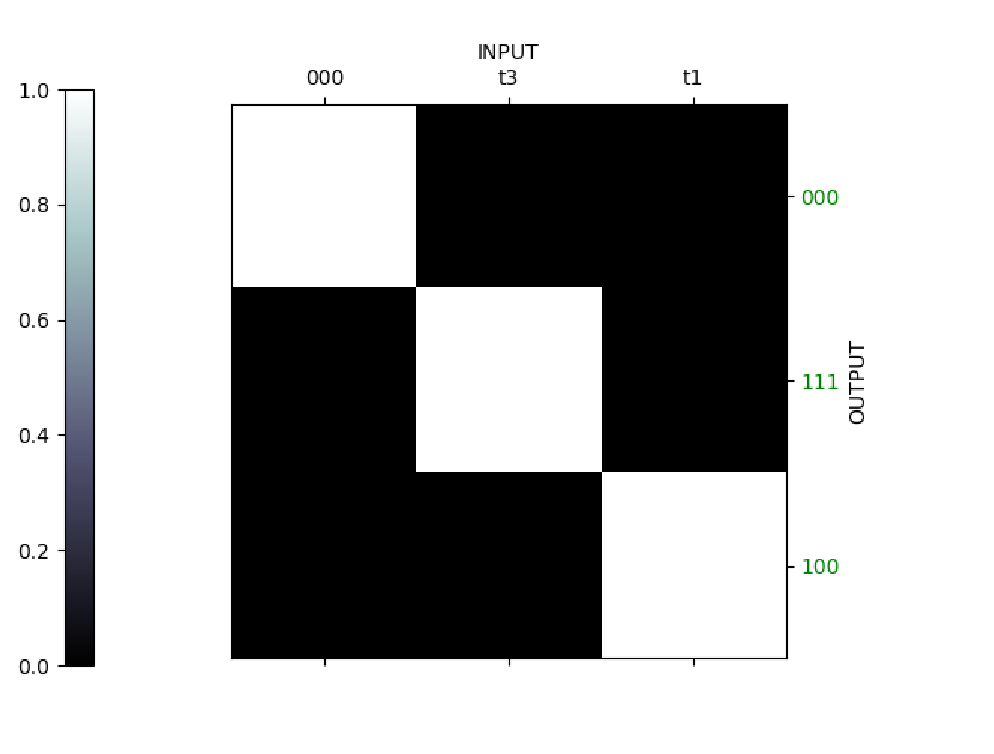
\includegraphics[width=\linewidth,keepaspectratio=true]{./figs/lookup/lt-trace-eps}
		\fi
		\caption{AG Trace for Lookup Tables}
		\label{ag_lt}
	\end{minipage}
\end{figure}


\subsection{Accuracy}
Since the lookup tables can be viewed as nested functions, accuracy of final output of the composition can be an adequate measure of model performance. However since we want to ensure that the model doesn't learn spurious patterns in data to land at an un-compositional solution, we want it to be accurate at each step of the composition. This hierarchical measure of accuracy is a viable test for the compositionality of the network. Therefore in all evaluations \textit{sequence accuracy} is the performance metric of the model.

\subparagraph{Hyperparameters}: Based on the hyperparameter grid search conducted by \cite{Hupkes2018} I ran the experiments with the best hyperparameters for both baseline (RNN cell=GRU, Embedding size=128, Hidden layer size=512, optimizer=Adam \citep{KingmaB14}, learning rate=0.001, attention=pre-rnn \citep{Bahdanau2014}, alignment measure=mlp(section \ref{mtv:attn})).

\subsection{Lookup Tables - Results}
\begin{figure}[ht] 
	\begin{subfigure}[b]{0.5\linewidth}
		\centering
		\ifpdf
		\includegraphics[width=0.95\linewidth]{./figs/lookup/baseline-loss-pdf}
		\else
		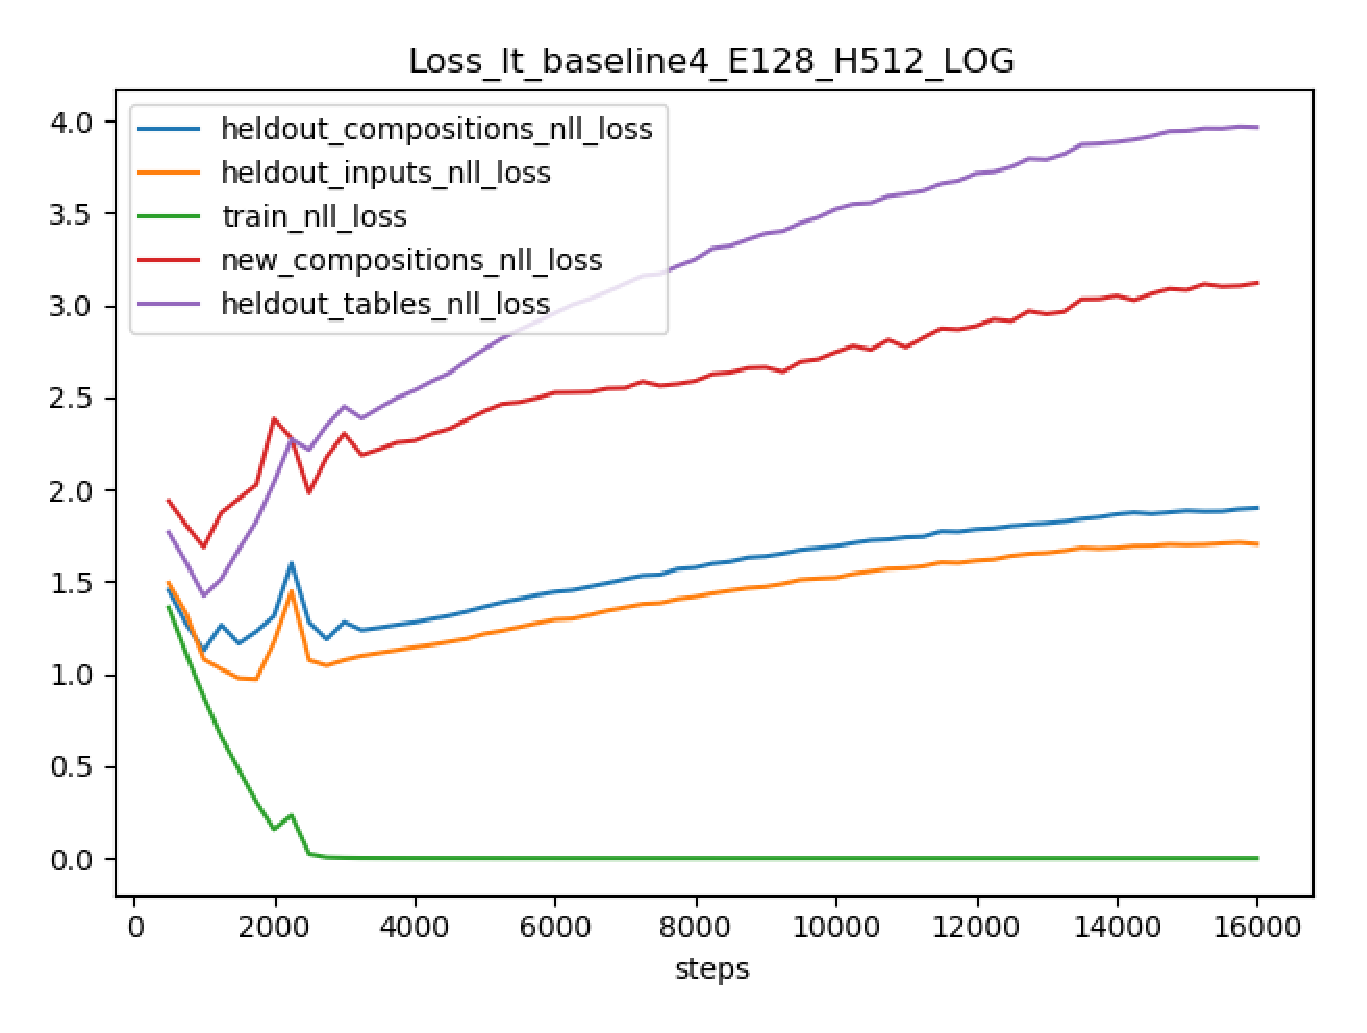
\includegraphics[width=0.95\linewidth]{./figs/lookup/baseline-loss-eps}
		\fi
		\caption{Loss Curves for Baseline} 
		\label{lt_baseline} 
		\vspace{2ex}
	\end{subfigure}%% 
	\begin{subfigure}[b]{0.5\linewidth}
		\centering
		\ifpdf
		\includegraphics[width=0.95\linewidth]{./figs/lookup/learned-loss-pdf}
		\else
		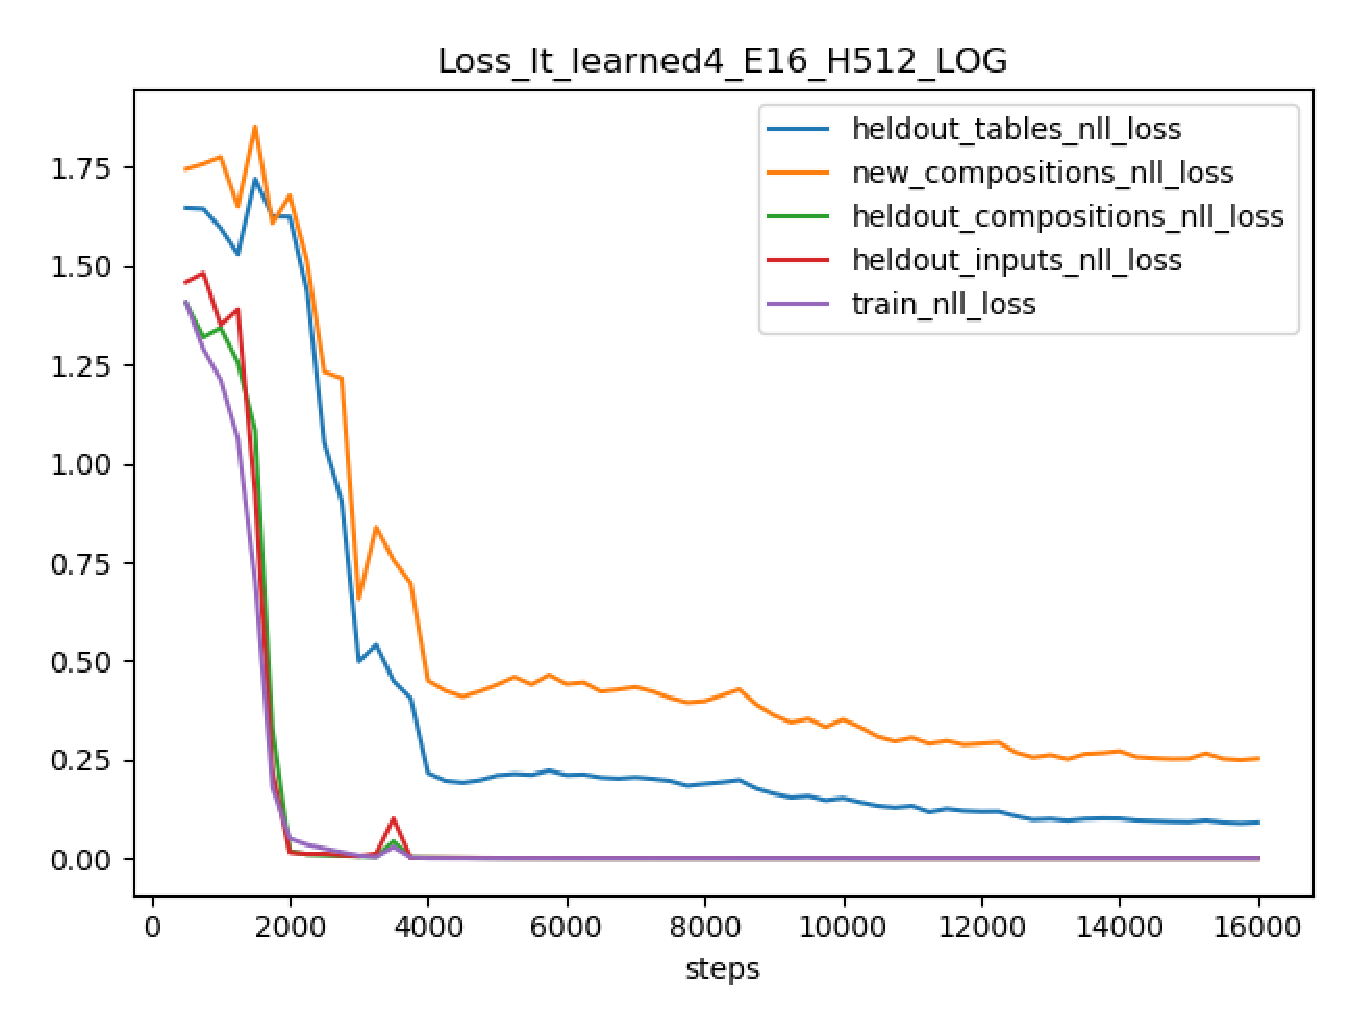
\includegraphics[width=0.95\linewidth]{./figs/lookup/learned-loss-eps}
		\fi 
		\caption{Loss Curves for Learned} 
		\label{lt_learned} 
		\vspace{2ex}
	\end{subfigure}
		\caption{Learning Curves for Lookup Tables}
		\label{lt_learning_curves}
\end{figure}
			
\begin{figure}
	\begin{minipage}[t]{\textwidth}
		\ifpdf
		\includegraphics[width=\linewidth,keepaspectratio=true]{./figs/lookup/lt-acc-pdf}
		\else
		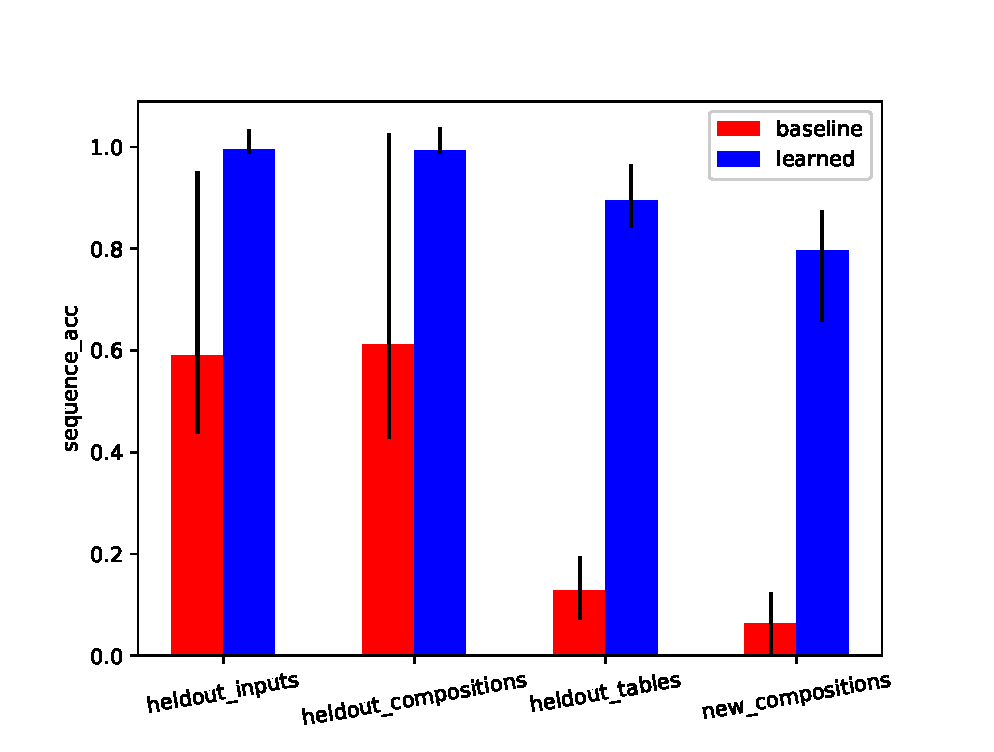
\includegraphics[width=\linewidth,keepaspectratio=true]{./figs/lookup/lt-acc-eps}
		\fi
		\caption{\small Average Sequence Accuracies}
		\label{res:lt-acc}
	\end{minipage}
\end{figure}


\section{Symbol Rewriting} \label{datasets:sr}
Introduced by \cite{Weber2018} the symbol rewriting dataset is essentially a probabilistic context free grammar (PCFG). It consists of a rewriting a set of input symbols to a set of output symbols based on this grammar. Before proceeding further with the task description,I'll elaborate on PCGFs briefly.

\subparagraph{PCFGs} are the stochastic version of CFGs (Context free grammars) that we encountered in section \ref{flt:ch}. The addition of this stochasticity was motivated by the non-uniformity of words in natural language. Assigning probabilities to production rules, lead to a grammar more in line with the Zipfian distribution of words in natural language \citep{jurafsky2014speech}. A PCFG consists of:

\begin{enumerate}
	\item A CFG $\mathcal{G} = \langle \Sigma, N, S, R \rangle$ where the symbols have the same meaning as defined in section \ref{flt}.
	\item A probability parameter $p(a \rightarrow b) \mid \displaystyle \sum_{a \rightarrow b \mid a \in N} p(a \rightarrow b) = 1 $ 
	\item $\therefore$ the probabilities associated with all the expansion rules of a given non-terminal should sum up to 1.
\end{enumerate}

The parse tree shown in figure \ref{figid} illustrates the production rule for one input symbol. The grammar consists of 41 such symbols each following similar production rules. \cite{Weber2018} showed using this dataset while seq2seq models are powerful enough to learn some structure from this data and generalize on a test set which was drawn from the same distribution as the training set. They posit that given the simplicity of the grammar it should be possible to generalize to test sets (with some hyperparameter tuning) that are atypical of the training distribution while still conforming to the underlying grammar. They however show that this indeed \textbf{is not} the case.

\subsection{Data Structure}
The data-splits as furnished \citep{Weber2018} consists of a training data and different test cases which are non-exhaustive and created by sampling randomly from all possible i/o pairs as described by the PCFG. The different test sets are created to ascertain if the seq2seq models actually understand the underlying grammar from the training data or simply memorize some spurious structure from the training distribution. For hyperparameter tuning a validation set which is an amalgamation of random samples from all the different test sets, is used. The details of the different data splits are presented below. Examples from each split and the size of each split are presented in table \ref{sr:stats}
\begin{enumerate}
	\item \textbf{train} consists of 100000 pairs of input output symbols with input string length ranging between $\langle$ 5 and 10 $\rangle$. Output string length is therefore between $\langle$ 15 and 30 $\rangle$. A crucial feature of this set is that no symbol is repeated in a given input string.
	\item \textbf{standard test} consists of samples drawn from the same distribution as the training set.
	\item \textbf{repeat test} includes input strings where repetition of symbols is allowed.
	\item \textbf{short test} includes input strings which are shorter in length as compared to the input strings in the training data. The input string length ranges between $\langle$ 1 and 4 $\rangle$.
	\item \textbf{long test} consists of input sequences of lengths in the range $\langle$ 11 and 15 $\rangle$.
\end{enumerate}

\begin{table}[ht]
	\centering
	\begin{tabular}{l|lc}
		& Example & Size\\
		\hline
		train & HS E I G DS  & 100000 \\
		standard test & LS KS G E C P T & 2000 \\
		repeat & I I I I I I MS & 2000 \\
		short & M I C & 2000 \\
		long & Y W G Q V I FS GS C JS R B E M KS & 2000 \\
	\end{tabular}
	\caption{Symbol Rewriting Splits}
	\label{sr:stats}
\end{table}

The datasets \textit{repeat, short and long} come from distributions which are different from the training distribution on which the model has learned the data structure. It is expected of a compositional learner that given the sufficient size of the training data it would be able to infer a pattern which is close to the underlying PCFG and therefore generalize of the test sets which comes from different distributions but have the same underlying structure.

\subsection{AG Trace}
\begin{figure}
	\begin{minipage}[t]{\textwidth}
		\ifpdf
		\includegraphics[width=\linewidth,keepaspectratio=true]{./figs/lookup/sr-trace-pdf}
		\else
		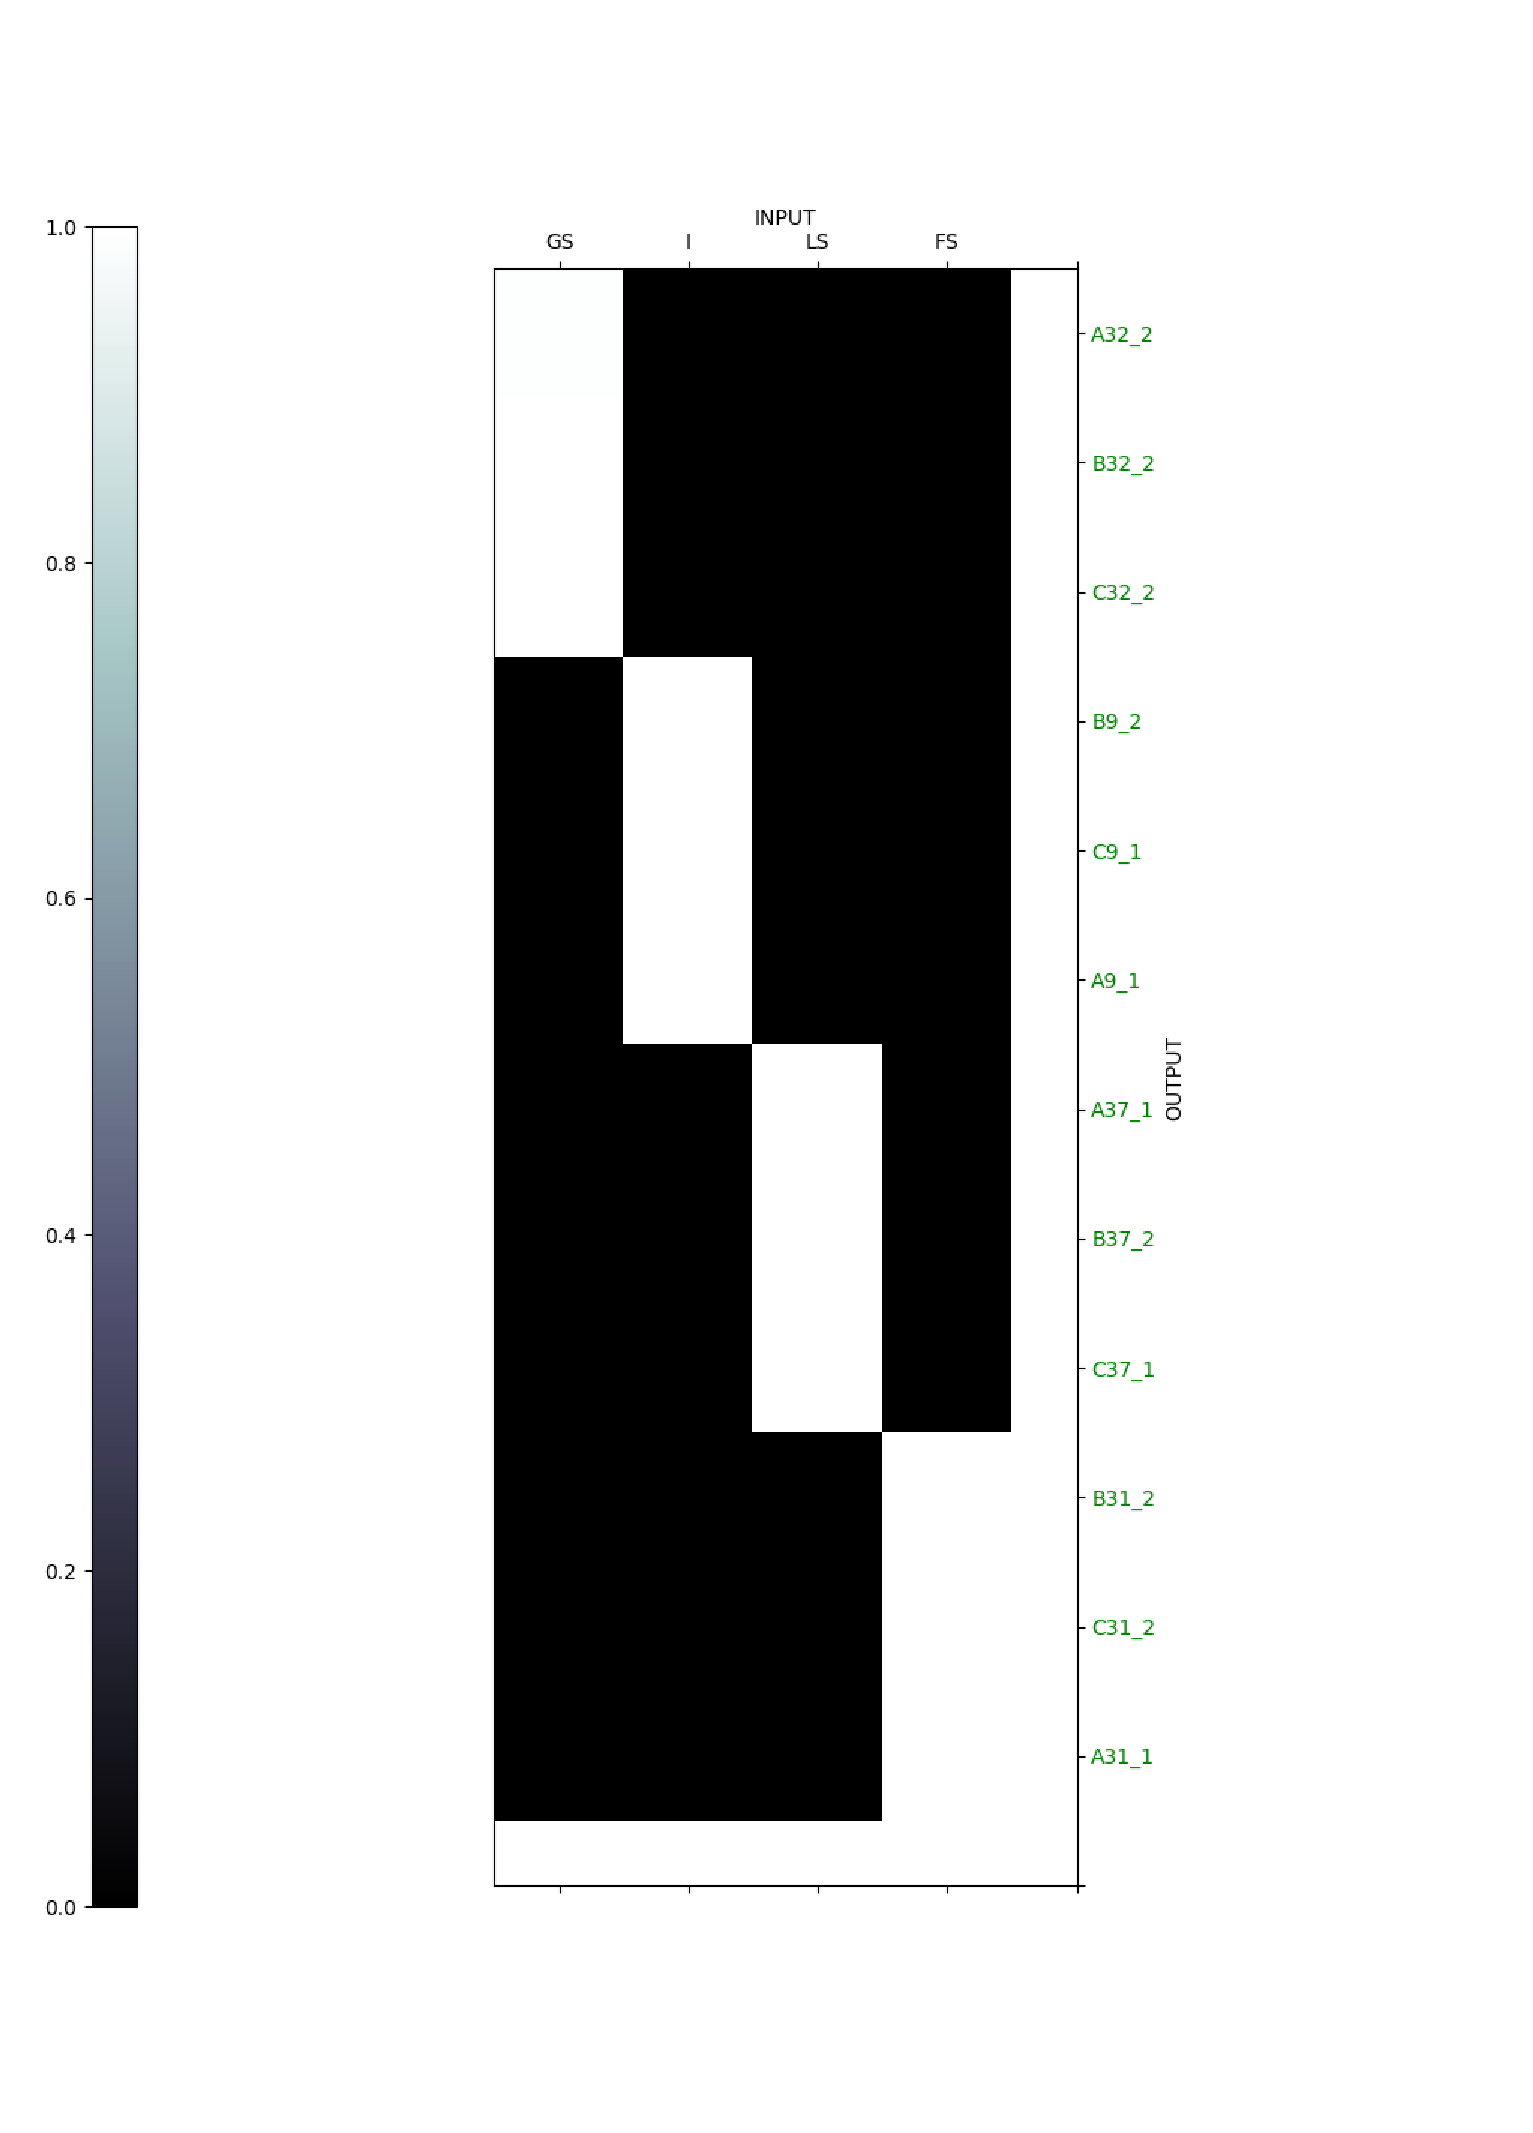
\includegraphics[width=\linewidth,keepaspectratio=true]{./figs/lookup/sr-trace-eps}
		\fi
		\caption{AG Trace for Symbol rewriting}
		\label{lt_sr_trace}
	\end{minipage}
\end{figure}
